\documentclass{standalone}

\usepackage{pgfplots,siunitx}
\pgfplotsset{compat=newest}

\AtBeginDocument{\renewcommand{\AtBeginDocument}[1]{}}

\begin{document}

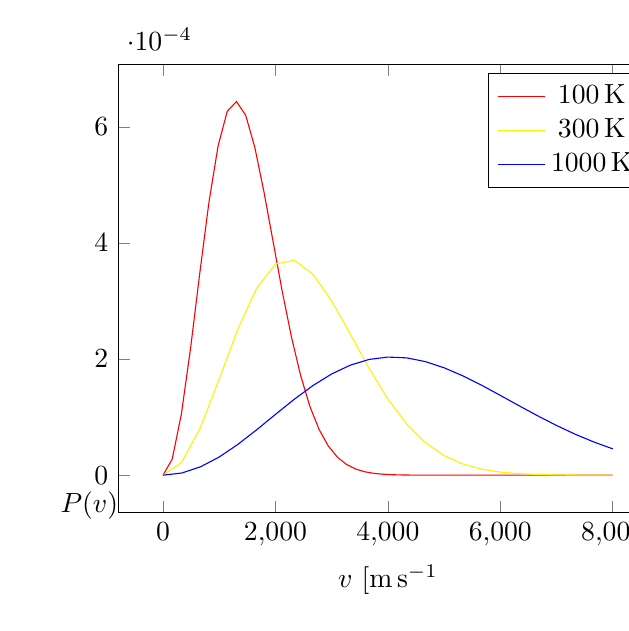
\begin{tikzpicture}

  \def\kB{1.3806488e-23} % Boltzmann constant
  \def\mu{1.660538921e-27} % unified atomic mass unit/Dalton (symbols: m_u or Da)
  \def\w#1{4 * pi * (\mu / (2 * pi * \kB * #1))^(3/2) * x^2 * exp(-\mu * x^2 / (2 * \kB * #1))}

  \begin{axis}[
      domain = 0:8000,
      xlabel = $v$ [\si{\metre\per\second}],
      ylabel = $P(v)$,
      smooth, thick,
      axis lines = left,
      every tick/.style = {thick}
    ]

    \addplot[color=red,samples = 50]{\w{100}};

    \addplot[color=yellow]{\w{300}};

    \addplot[color=blue]{\w{1000}};

    \legend{\SI{100}{\kelvin}, \SI{300}{\kelvin}, \SI{1000}{\kelvin}}

  \end{axis}
\end{tikzpicture}

\end{document}